One of the goals of this thesis was to visualize the structure of the scraped portion of the dark web. We chose to render the data as a web graph which is further outlined in section~\ref{webGraph}. As was described in chapter~\ref{datasetAnalysis}, the data set to be displayed was rather sizable. The problem with the visualization of such an amount of data is readability. All pages of such a data set cannot be displayed at the same time if additional information, such as the category with the url address of the page, needs to be provided to the user. Such rendering would be cluttered and readability would be affected negatively. It was therefore necessary to find a proper way to divide the graph into several subgraphs. We decided to adopt community structure introduced in section~\ref{communityStructure}. For community detection we leveraged the well known Louvain algorithm (LA). LA is described in more detail in section~\ref{louvainAlgorithm}.

In this chapter we characterize web graphs and its challenges. Next we talk about community structure and LA, the algorithm for dividing a graph into communities. 
 
\section{Web graph} \label{webGraph}
The data is displayed as a graph. More precisely a web graph~\cite{the_web_graph_overview}. A web graph is a graph representation of the web. Nodes are portrayals of the pages and edges depict links between the pages. Web graphs tend to be built from an enormous amount of data. As such, they can be advertised in various ways. One of the visualizations is shown in figure~\ref{hugeWebGraphFireworks}. 
\begin{figure}[ht!]
  \centering
  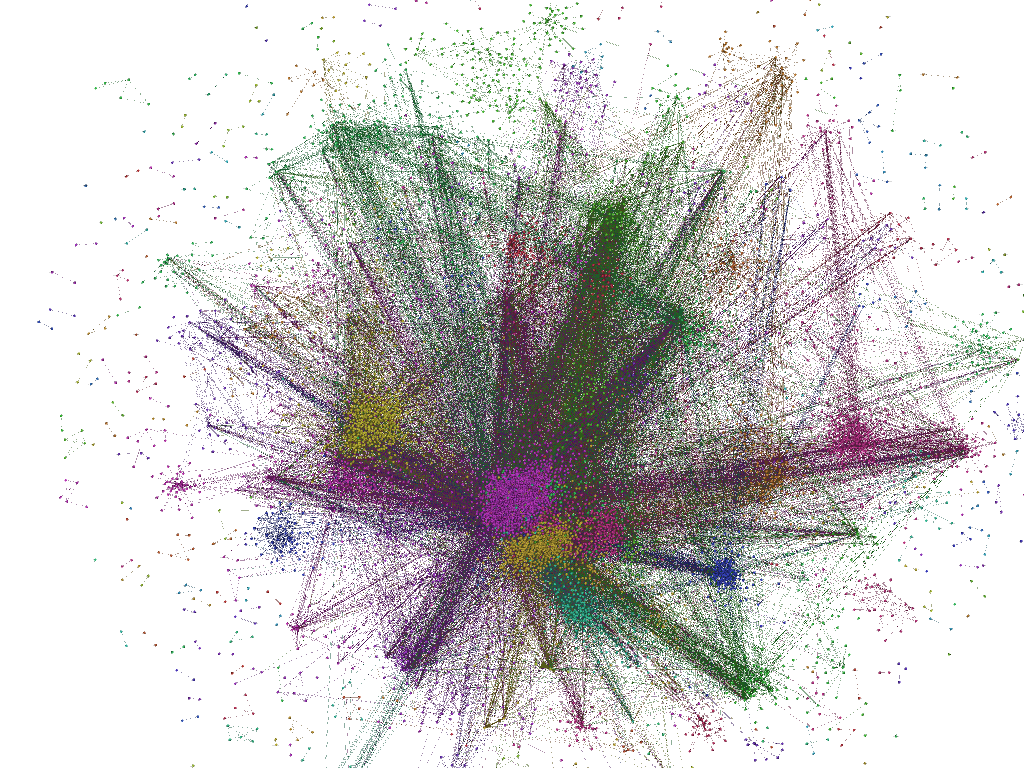
\includegraphics[width=\textwidth]{Images/hugeWebGraphFireworks.png}
  \caption{Web graph by Citeo made consisting of circa 600 000 domains and 16 billion links.~\cite{hugeWebGraphFireworks}.}
  \label{hugeWebGraphFireworks}
\end{figure} 
The depicted web graph displays all its data at once without any labels or details. The result may be useful for viewing the internet as a whole. However, for our purposes this view was not sufficient. One of the requirements of this thesis was the possibility of the inspection of the relationships between nodes in more detail. The big amount of data described in subsection~\ref{dataSet} prevented the displaying of all pages at once. The information the user would read from such a graph would be either incompatible with the requirements or incomprehensible as too much visual data worsens the quality of the user's information processing~\cite{informationCluttering}. Therefore the requirement arose for the graph to be composed of a significantly smaller amount of nodes. As a result the user would be able to obtain the sought knowledge without hindrances. The majority of the nodes in our graph were not isolated\footnote{An isolated node is a node with zero incoming and outgoing edges.}. The nodes were in fact part of a single connected component. It was therefore possible to partition the graph based on the density of its nodes into communities. Communities are described in detail in the next subsection~\ref{communityStructure}.

\subsection{Community structure} \label{communityStructure}
If a graph can be partitioned into several subgraphs so that nodes from one subgraph are internally connected densely and are connected scarcely to nodes from other subgraphs, we can claim it has a community structure. Each subgraph of such a graph is a community~\cite{communitiesOverview}. Each community can be portrayed as a meta node of the graph. This way the number of nodes in the graph is reduced. The quality of such a partition is measured using modularity. L. Wenye and D. Schuurmans describe modularity in their work~\cite{modularityOverview} with the following words: \begin{quotation}  For a candidate partition of the vertices into clusters, the modularity is defined to be the portion of the edge connections within the same cluster minus the expected portion if the connections were distributed randomly~\cite{modularityDefinition}. \end{quotation}

\section{Louvain algorithm} \label{louvainAlgorithm}
A widely used algorithm for finding communities in graphs is LA~\cite{louvainAlgorithm}. It is a greedy algorithm which maximizes modularity locally. The modularity value is a number between -1 and 1. Next we detail the principle of the algorithm. We example each step on node $N_{A}$ belonging to a part of an example graph illustrated in figure \ref{exampleGraphLouvain}.
\begin{figure}[ht!]
  \centering
  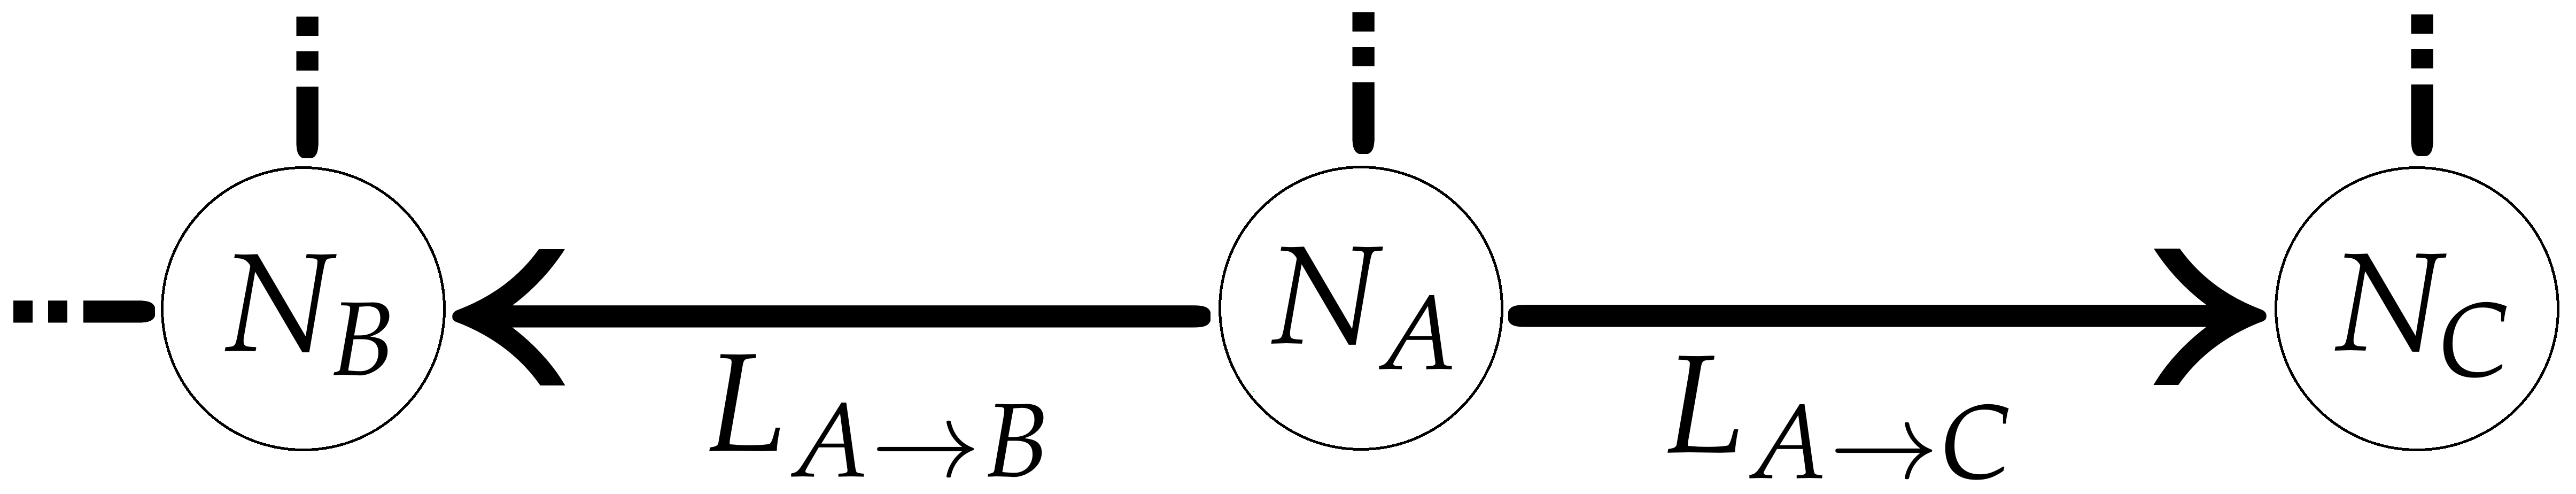
\includegraphics[width=\textwidth]{Images/graphForCommunity.png}
  \caption{The visible portion of the exampled graph depicts nodes $N_{A}$, $N_{B}$, and  node $N_{C}$. There are links  $L_{A\rightarrow B}$ and  $L_{A\rightarrow C}$  between nodes  $N_{A}$ and  $N_{B}$, and  $N_{A}$ and  $N_{C}$ respectively. Other links are displayed partially and are connecting the nodes to the rest of the graph.}
  \label{exampleGraphLouvain}
\end{figure} 

\begin{enumerate} 
  \label{louvainAlgorithmPrinciple}
  \item  Each node is assigned a community. Current modularity for each node is calculated. 
  \begin{itemize}
    \item Node $N_{A}$ is assigned to community $C_{A}$.The modularity value $M_{A\rightarrow cA}$ for $N_{A}$ is \textit{0.2}.
  \end{itemize} 
  \item Each node is disassociated from its community and randomly appointed to a community of one of its neighbours. This is repeated for each neighbour of the node. Modularity for each node after each such a transition is calculated.
  \begin{itemize}
    \item Node $N_{A}$ has two neighbouring nodes, node $N_{B}$ in the community $C_{B}$ and node $N_{C}$ in the community $C_{C}$. Node $N_{A}$ is removed from $C_{A}$ and appointed to $C_{B}$. Modularity value $M_{A\rightarrow cB}$ is \textit{-0.1}. Afterwards, $N_{A}$ is removed from $C_{B}$ and assigned to $C_{C}$. Modularity value $M_{A\rightarrow cC}$ is \textit{0.5}. 
  \end{itemize} 
  \item Each node is now appointed to the community in which the maximum modularity value was achieved. This can also result in the node remaining in its original community.
  \begin{itemize}
    \item The maximum modularity of $N_{A}$ achieved in the previous step is $M_{A\rightarrow cC}$. $N_{A}$ is therefore removed from $C_{A}$ and appointed to $C_{C}$.
  \end{itemize} 
  \item Discard the empty communities. 
  \begin{itemize}
    \item Community $C_{A}$ is now empty and is therefore discarded.
  \end{itemize} 
  \item Each community is now considered a node (community-node). Links between community-nodes are constructed from links of nodes of the same community-node (old-links). This is done by grouping together old-links which target nodes assigned to the same target community-node. These grouped links now represent weighed edges between community-nodes. Old links between nodes of the same community-node are represented  by a self-loop on the community-node.
  \begin{itemize}
    \item Community $C_{C}$ is now considered a node $N_{cC}$ and $C_{B}$ is considered a node $N_{cB}$. A link $L_{cC\rightarrow cB}$ from $N_{cC}$ to $N_{cB}$ with a weight of 1 is created because  of link $L_{A\rightarrow B}$. Also, a loop $L_{cC\rightarrow cC}$ is created on $N_{cC}$ because of the link $L_{A\rightarrow C}$. The result of this step can be observed in figure \ref{exampleGraphLouvainEnde}.
  \end{itemize}  
\begin{figure}[ht!]
  \centering
  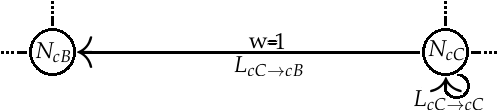
\includegraphics[width=\textwidth]{Images/graphForCommunityEnde.png}
  \caption{This graph is the result of applying the above listed steps to the previously shown portion of the example graph from figure \ref{exampleGraphLouvain}. The visible portion of the graph contains nodes $N_{cB}$ and $N_{cC}$, and a link $L_{cC\rightarrow cB}$ with a weight of 1 between them. A self-loop $L_{cC\rightarrow cC}$ on $N_{cC}$ is present.}
  \label{exampleGraphLouvainEnde}
\end{figure} 
    
\end{enumerate}
LA is favoured for its simplicity, speed and accuracy. Since its introduction, in 2008, it was possible to detect communities in graphs with billions of nodes in a relatively timely manner. LA was compared to other algorithms for community detection \cite{louvainAlgorithm}.  Namely the algorithm of Wakita and Tsurumi \cite{wakitaAndToshiyuki}, of Pons and Latapy \cite{ponsAndLatapy}, and of Clauset, Newman and Moore \cite{CNM}. The used graphs were of sizes varying between 34 nodes and 77 edges to as much as 118 million nodes and 1 billion edges. The difference between the computing times of the previously stated algorithms grows with the size of the graphs and favours LA. In fact, it took 152 minutes for LA to detect the communities of the greatest graph whereas the computation time of the other algorithms was more than 24 hours. In terms of precision, LA was also the most precise one with slightly better modularities.

